\documentclass[]{book}
\usepackage{lmodern}
\usepackage{amssymb,amsmath}
\usepackage{ifxetex,ifluatex}
\usepackage{fixltx2e} % provides \textsubscript
\ifnum 0\ifxetex 1\fi\ifluatex 1\fi=0 % if pdftex
  \usepackage[T1]{fontenc}
  \usepackage[utf8]{inputenc}
\else % if luatex or xelatex
  \ifxetex
    \usepackage{mathspec}
  \else
    \usepackage{fontspec}
  \fi
  \defaultfontfeatures{Ligatures=TeX,Scale=MatchLowercase}
\fi
% use upquote if available, for straight quotes in verbatim environments
\IfFileExists{upquote.sty}{\usepackage{upquote}}{}
% use microtype if available
\IfFileExists{microtype.sty}{%
\usepackage{microtype}
\UseMicrotypeSet[protrusion]{basicmath} % disable protrusion for tt fonts
}{}
\usepackage[margin=1in]{geometry}
\usepackage{hyperref}
\hypersetup{unicode=true,
            pdftitle={A Minimal Book Example},
            pdfauthor={Yihui Xie},
            pdfborder={0 0 0},
            breaklinks=true}
\urlstyle{same}  % don't use monospace font for urls
\usepackage{natbib}
\bibliographystyle{apalike}
\usepackage{color}
\usepackage{fancyvrb}
\newcommand{\VerbBar}{|}
\newcommand{\VERB}{\Verb[commandchars=\\\{\}]}
\DefineVerbatimEnvironment{Highlighting}{Verbatim}{commandchars=\\\{\}}
% Add ',fontsize=\small' for more characters per line
\usepackage{framed}
\definecolor{shadecolor}{RGB}{248,248,248}
\newenvironment{Shaded}{\begin{snugshade}}{\end{snugshade}}
\newcommand{\KeywordTok}[1]{\textcolor[rgb]{0.13,0.29,0.53}{\textbf{#1}}}
\newcommand{\DataTypeTok}[1]{\textcolor[rgb]{0.13,0.29,0.53}{#1}}
\newcommand{\DecValTok}[1]{\textcolor[rgb]{0.00,0.00,0.81}{#1}}
\newcommand{\BaseNTok}[1]{\textcolor[rgb]{0.00,0.00,0.81}{#1}}
\newcommand{\FloatTok}[1]{\textcolor[rgb]{0.00,0.00,0.81}{#1}}
\newcommand{\ConstantTok}[1]{\textcolor[rgb]{0.00,0.00,0.00}{#1}}
\newcommand{\CharTok}[1]{\textcolor[rgb]{0.31,0.60,0.02}{#1}}
\newcommand{\SpecialCharTok}[1]{\textcolor[rgb]{0.00,0.00,0.00}{#1}}
\newcommand{\StringTok}[1]{\textcolor[rgb]{0.31,0.60,0.02}{#1}}
\newcommand{\VerbatimStringTok}[1]{\textcolor[rgb]{0.31,0.60,0.02}{#1}}
\newcommand{\SpecialStringTok}[1]{\textcolor[rgb]{0.31,0.60,0.02}{#1}}
\newcommand{\ImportTok}[1]{#1}
\newcommand{\CommentTok}[1]{\textcolor[rgb]{0.56,0.35,0.01}{\textit{#1}}}
\newcommand{\DocumentationTok}[1]{\textcolor[rgb]{0.56,0.35,0.01}{\textbf{\textit{#1}}}}
\newcommand{\AnnotationTok}[1]{\textcolor[rgb]{0.56,0.35,0.01}{\textbf{\textit{#1}}}}
\newcommand{\CommentVarTok}[1]{\textcolor[rgb]{0.56,0.35,0.01}{\textbf{\textit{#1}}}}
\newcommand{\OtherTok}[1]{\textcolor[rgb]{0.56,0.35,0.01}{#1}}
\newcommand{\FunctionTok}[1]{\textcolor[rgb]{0.00,0.00,0.00}{#1}}
\newcommand{\VariableTok}[1]{\textcolor[rgb]{0.00,0.00,0.00}{#1}}
\newcommand{\ControlFlowTok}[1]{\textcolor[rgb]{0.13,0.29,0.53}{\textbf{#1}}}
\newcommand{\OperatorTok}[1]{\textcolor[rgb]{0.81,0.36,0.00}{\textbf{#1}}}
\newcommand{\BuiltInTok}[1]{#1}
\newcommand{\ExtensionTok}[1]{#1}
\newcommand{\PreprocessorTok}[1]{\textcolor[rgb]{0.56,0.35,0.01}{\textit{#1}}}
\newcommand{\AttributeTok}[1]{\textcolor[rgb]{0.77,0.63,0.00}{#1}}
\newcommand{\RegionMarkerTok}[1]{#1}
\newcommand{\InformationTok}[1]{\textcolor[rgb]{0.56,0.35,0.01}{\textbf{\textit{#1}}}}
\newcommand{\WarningTok}[1]{\textcolor[rgb]{0.56,0.35,0.01}{\textbf{\textit{#1}}}}
\newcommand{\AlertTok}[1]{\textcolor[rgb]{0.94,0.16,0.16}{#1}}
\newcommand{\ErrorTok}[1]{\textcolor[rgb]{0.64,0.00,0.00}{\textbf{#1}}}
\newcommand{\NormalTok}[1]{#1}
\usepackage{longtable,booktabs}
\usepackage{graphicx,grffile}
\makeatletter
\def\maxwidth{\ifdim\Gin@nat@width>\linewidth\linewidth\else\Gin@nat@width\fi}
\def\maxheight{\ifdim\Gin@nat@height>\textheight\textheight\else\Gin@nat@height\fi}
\makeatother
% Scale images if necessary, so that they will not overflow the page
% margins by default, and it is still possible to overwrite the defaults
% using explicit options in \includegraphics[width, height, ...]{}
\setkeys{Gin}{width=\maxwidth,height=\maxheight,keepaspectratio}
\IfFileExists{parskip.sty}{%
\usepackage{parskip}
}{% else
\setlength{\parindent}{0pt}
\setlength{\parskip}{6pt plus 2pt minus 1pt}
}
\setlength{\emergencystretch}{3em}  % prevent overfull lines
\providecommand{\tightlist}{%
  \setlength{\itemsep}{0pt}\setlength{\parskip}{0pt}}
\setcounter{secnumdepth}{5}
% Redefines (sub)paragraphs to behave more like sections
\ifx\paragraph\undefined\else
\let\oldparagraph\paragraph
\renewcommand{\paragraph}[1]{\oldparagraph{#1}\mbox{}}
\fi
\ifx\subparagraph\undefined\else
\let\oldsubparagraph\subparagraph
\renewcommand{\subparagraph}[1]{\oldsubparagraph{#1}\mbox{}}
\fi

%%% Use protect on footnotes to avoid problems with footnotes in titles
\let\rmarkdownfootnote\footnote%
\def\footnote{\protect\rmarkdownfootnote}

%%% Change title format to be more compact
\usepackage{titling}

% Create subtitle command for use in maketitle
\newcommand{\subtitle}[1]{
  \posttitle{
    \begin{center}\large#1\end{center}
    }
}

\setlength{\droptitle}{-2em}
  \title{A Minimal Book Example}
  \pretitle{\vspace{\droptitle}\centering\huge}
  \posttitle{\par}
  \author{Yihui Xie}
  \preauthor{\centering\large\emph}
  \postauthor{\par}
  \predate{\centering\large\emph}
  \postdate{\par}
  \date{2018-06-28}

\usepackage{booktabs}

\usepackage{amsthm}
\newtheorem{theorem}{Theorem}[chapter]
\newtheorem{lemma}{Lemma}[chapter]
\theoremstyle{definition}
\newtheorem{definition}{Definition}[chapter]
\newtheorem{corollary}{Corollary}[chapter]
\newtheorem{proposition}{Proposition}[chapter]
\theoremstyle{definition}
\newtheorem{example}{Example}[chapter]
\theoremstyle{definition}
\newtheorem{exercise}{Exercise}[chapter]
\theoremstyle{remark}
\newtheorem*{remark}{Remark}
\newtheorem*{solution}{Solution}
\begin{document}
\maketitle

{
\setcounter{tocdepth}{1}
\tableofcontents
}
\chapter{Prerequisites}\label{prerequisites}

This is a \emph{sample} book written in \textbf{Markdown}. You can use
anything that Pandoc's Markdown supports, e.g., a math equation
\(a^2 + b^2 = c^2\).

The \textbf{bookdown} package can be installed from CRAN or Github:

\begin{Shaded}
\begin{Highlighting}[]
\KeywordTok{install.packages}\NormalTok{(}\StringTok{"bookdown"}\NormalTok{)}
\CommentTok{# or the development version}
\CommentTok{# devtools::install_github("rstudio/bookdown")}
\end{Highlighting}
\end{Shaded}

Remember each Rmd file contains one and only one chapter, and a chapter
is defined by the first-level heading \texttt{\#}.

To compile this example to PDF, you need XeLaTeX. You are recommended to
install TinyTeX (which includes XeLaTeX):
\url{https://yihui.name/tinytex/}.

\chapter{Reading Data into R}\label{reading-data-into-r}

The first step in every analysis requires data to be read into the
environment, and learning how to do this is the first hurdle a person
needs to overcome to begin learning to use R.

In this chapter, we will first discuss how to read data using functions
in Base-R (when possible), and then we will discuss alternative
packages, such as the multitude of packages in the
\href{https://www.tidyverse.org}{Tidyverse}, and highlight their
advantages over Base-R functions.

\begin{itemize}
\tightlist
\item
  \includegraphics{https://github.com/tidyverse/haven/blob/master/man/figures/logo.png}
\end{itemize}

\section{The Many Formats of Data
Files}\label{the-many-formats-of-data-files}

Data can exist in many different formats, either as the generic
universal types (e.g.~csv, tsv, .json, etc) or software specific types
(e.g. \texttt{.xlsx}, `` )

\subsection{File-based Data}\label{file-based-data}

\subsubsection{Generic Formats}\label{generic-formats}

\paragraph{CSV- Comma Separated
Values}\label{csv--comma-separated-values}

The fields are separated by a comma \texttt{,} and are typically used
for loading into spreadsheets.

For example:

\begin{Shaded}
\begin{Highlighting}[]
\NormalTok{csv_example_path <-}\StringTok{ "data/ASCII-comma/FEV.DAT.txt"}

\KeywordTok{readLines}\NormalTok{(csv_example_path)[}\DecValTok{1}\OperatorTok{:}\DecValTok{8}\NormalTok{]  }\CommentTok{# reads each line of the file}
\end{Highlighting}
\end{Shaded}

\begin{verbatim}
[1] "'Id','Age','FEV','Hgt','Sex','Smoke'"
[2] "301,9,1.708,57,0,0"                  
[3] "451,8,1.724,67.5,0,0"                
[4] "501,7,1.72,54.5,0,0"                 
[5] "642,9,1.558,53,1,0"                  
[6] "901,9,1.895,57,1,0"                  
[7] "1701,8,2.336,61,0,0"                 
[8] "1752,6,1.919,58,0,0"                 
\end{verbatim}

\begin{Shaded}
\begin{Highlighting}[]
\CommentTok{# Note: readLines(csv_example_path) is the same as}
\CommentTok{# readLines("data/ASCII-comma/FEV.DAT.txt")}
\end{Highlighting}
\end{Shaded}

In Base-R, CSV data can be read using the \texttt{read.csv()} function.
The \texttt{read.csv2()} function is used in countires that use a comma
as a decimal point and a semicolon as a field separator.

\begin{Shaded}
\begin{Highlighting}[]
\NormalTok{csv_example <-}\StringTok{ }\KeywordTok{read.csv}\NormalTok{(csv_example_path)}

\KeywordTok{head}\NormalTok{(csv_example)}
\end{Highlighting}
\end{Shaded}

\begin{verbatim}
  X.Id. X.Age. X.FEV. X.Hgt. X.Sex. X.Smoke.
1   301      9  1.708   57.0      0        0
2   451      8  1.724   67.5      0        0
3   501      7  1.720   54.5      0        0
4   642      9  1.558   53.0      1        0
5   901      9  1.895   57.0      1        0
6  1701      8  2.336   61.0      0        0
\end{verbatim}

\paragraph{TSV- Tab Separeted Values}\label{tsv--tab-separeted-values}

The fields are separated by a tabulation or \t and are saved as
\texttt{.txt} files. However, not all \texttt{.txt} files contain tab
separated values.

For example:

\begin{Shaded}
\begin{Highlighting}[]
\NormalTok{tsv_example_path <-}\StringTok{ "data/ASCII-tab/FEV.DAT.txt"}

\KeywordTok{readLines}\NormalTok{(tsv_example_path)[}\DecValTok{1}\OperatorTok{:}\DecValTok{8}\NormalTok{]}
\end{Highlighting}
\end{Shaded}

\begin{verbatim}
[1] "'Id'\t'Age'\t'FEV'\t'Hgt'\t'Sex'\t'Smoke'"
[2] "301\t9\t1.708\t57\t0\t0"                  
[3] "451\t8\t1.724\t67.5\t0\t0"                
[4] "501\t7\t1.72\t54.5\t0\t0"                 
[5] "642\t9\t1.558\t53\t1\t0"                  
[6] "901\t9\t1.895\t57\t1\t0"                  
[7] "1701\t8\t2.336\t61\t0\t0"                 
[8] "1752\t6\t1.919\t58\t0\t0"                 
\end{verbatim}

\begin{Shaded}
\begin{Highlighting}[]
\NormalTok{tsv_example <-}\StringTok{ }\KeywordTok{read.delim}\NormalTok{(}\StringTok{"data/ASCII-tab/FEV.DAT.txt"}\NormalTok{)}
\KeywordTok{head}\NormalTok{(tsv_example)}
\end{Highlighting}
\end{Shaded}

\begin{verbatim}
  X.Id. X.Age. X.FEV. X.Hgt. X.Sex. X.Smoke.
1   301      9  1.708   57.0      0        0
2   451      8  1.724   67.5      0        0
3   501      7  1.720   54.5      0        0
4   642      9  1.558   53.0      1        0
5   901      9  1.895   57.0      1        0
6  1701      8  2.336   61.0      0        0
\end{verbatim}

\subsubsection{Excel}\label{excel}

\begin{Shaded}
\begin{Highlighting}[]
\KeywordTok{library}\NormalTok{(readxl)}
\end{Highlighting}
\end{Shaded}

\subsubsection{Software Specific
Formats}\label{software-specific-formats}

R is increasingly recognized as the gold standard for statistical
computations, yet some of your future collaboraters will exclusively use
Commercial Software (SAS, SPSS, Matlab, and Stata) for their statistical
computations. Although these individuals are limited by the types of
files they can read or write, the \texttt{haven} R-package can both read
and write any of these file formats.

\begin{Shaded}
\begin{Highlighting}[]
\KeywordTok{library}\NormalTok{(haven)}
\end{Highlighting}
\end{Shaded}

\paragraph{\texorpdfstring{SAS(\texttt{.sas7bdat}),
SPSS(\texttt{.sav},\texttt{.por}, \texttt{.xpt}), Stata
(\texttt{.dta})}{SAS(.sas7bdat), SPSS(.sav,.por, .xpt), Stata (.dta)}}\label{sas.sas7bdat-spss.sav.por-.xpt-stata-.dta}

\begin{Shaded}
\begin{Highlighting}[]
\NormalTok{sas <-}\StringTok{ }\KeywordTok{read_sas}\NormalTok{(}\StringTok{"data/SAS/FEV.sas7bdat"}\NormalTok{)}

\KeywordTok{head}\NormalTok{(sas)}
\end{Highlighting}
\end{Shaded}

\begin{verbatim}
# A tibble: 6 x 6
     ID   AGE   FEV   HGT   SEX SMOKE
  <dbl> <dbl> <dbl> <dbl> <dbl> <dbl>
1   301     9  1.71  57       0     0
2   451     8  1.72  67.5     0     0
3   501     7  1.72  54.5     0     0
4   642     9  1.56  53       1     0
5   901     9  1.90  57       1     0
6  1701     8  2.34  61       0     0
\end{verbatim}

\begin{Shaded}
\begin{Highlighting}[]
\NormalTok{spss <-}\StringTok{ }\KeywordTok{read_spss}\NormalTok{(}\StringTok{"data/SPSS/FEV.DAT.sav"}\NormalTok{)}
\KeywordTok{head}\NormalTok{(spss)}
\end{Highlighting}
\end{Shaded}

\begin{verbatim}
# A tibble: 6 x 6
     Id   Age   FEV   Hgt   Sex Smoke
  <dbl> <dbl> <dbl> <dbl> <dbl> <dbl>
1   301     9  1.71  57       0     0
2   451     8  1.72  67.5     0     0
3   501     7  1.72  54.5     0     0
4   642     9  1.56  53       1     0
5   901     9  1.90  57       1     0
6  1701     8  2.34  61       0     0
\end{verbatim}

\begin{Shaded}
\begin{Highlighting}[]
\NormalTok{stata <-}\StringTok{ }\KeywordTok{read_stata}\NormalTok{(}\StringTok{"data/Stata/FEV.DAT.dta"}\NormalTok{)}
\KeywordTok{head}\NormalTok{(stata)}
\end{Highlighting}
\end{Shaded}

\begin{verbatim}
# A tibble: 6 x 6
     Id   Age   fev   Hgt   Sex Smoke
  <dbl> <dbl> <dbl> <dbl> <dbl> <dbl>
1   301     9  1.71  57       0     0
2   451     8  1.72  67.5     0     0
3   501     7  1.72  54.5     0     0
4   642     9  1.56  53       1     0
5   901     9  1.90  57       1     0
6  1701     8  2.34  61       0     0
\end{verbatim}

The \texttt{foreign} package included in Base-R can also be used to
Reading and writing data stored by some versions of `Epi Info',
`Minitab', `S', `SAS', `SPSS', `Stata', `Systat', `Weka',and for reading
and writing some `dBase' files.

\paragraph{RDS}\label{rds}

\begin{Shaded}
\begin{Highlighting}[]
\NormalTok{rds_example <-}\StringTok{ }\KeywordTok{readRDS}\NormalTok{(}\StringTok{"data/RDS/BETACAR.DAT.rds"}\NormalTok{)}
\KeywordTok{head}\NormalTok{(rds_example)}
\end{Highlighting}
\end{Shaded}

\begin{verbatim}
# A tibble: 6 x 8
  `'Prepar'` `'Id'` `'Base1lvl'` `'Base2lvl'` `'Wk6lvl'` `'Wk8lvl'`
       <int>  <int>        <int>        <int>      <int>      <int>
1          1     71          298          116        174        178
2          1     73          124          146        294        278
3          1     80          176          200        276        286
4          1     83          116          180        164        238
5          1     90          152          142        290        300
6          1     92          106          106        246        206
# ... with 2 more variables: `'Wk10lvl'` <int>, `'Wk12lvl'` <int>
\end{verbatim}

\paragraph{\texorpdfstring{\texttt{rdata}}{rdata}}\label{rdata}

The \texttt{.rdata} format is R's specific format. Instead of using a
\texttt{read.\{something\}} function, \texttt{.rdata} is read into the
environment using \texttt{load(filename.rdata)} and retains the original
name it had when it was last saved.

\begin{Shaded}
\begin{Highlighting}[]
\KeywordTok{load}\NormalTok{(}\StringTok{"data/R/BETACAR.DAT.rdata"}\NormalTok{)  }\CommentTok{#named betacar when it was last saved}
\KeywordTok{head}\NormalTok{(betacar)}
\end{Highlighting}
\end{Shaded}

\begin{verbatim}
  Prepar Id Base1lvl Base2lvl Wk6lvl Wk8lvl Wk10lvl Wk12lvl
1      1 71      298      116    174    178     218     190
2      1 73      124      146    294    278     244     262
3      1 80      176      200    276    286     308     334
4      1 83      116      180    164    238     308     226
5      1 90      152      142    290    300     270     268
6      1 92      106      106    246    206     304     356
\end{verbatim}

\subsection{Directory-based Data}\label{directory-based-data}

\subsection{Database Connections}\label{database-connections}

\chapter{Introduction}\label{intro}

You can label chapter and section titles using \texttt{\{\#label\}}
after them, e.g., we can reference Chapter \ref{intro}. If you do not
manually label them, there will be automatic labels anyway, e.g.,
Chapter \ref{methods}.

Figures and tables with captions will be placed in \texttt{figure} and
\texttt{table} environments, respectively.

\begin{Shaded}
\begin{Highlighting}[]
\KeywordTok{par}\NormalTok{(}\DataTypeTok{mar =} \KeywordTok{c}\NormalTok{(}\DecValTok{4}\NormalTok{, }\DecValTok{4}\NormalTok{, .}\DecValTok{1}\NormalTok{, .}\DecValTok{1}\NormalTok{))}
\KeywordTok{plot}\NormalTok{(pressure, }\DataTypeTok{type =} \StringTok{'b'}\NormalTok{, }\DataTypeTok{pch =} \DecValTok{19}\NormalTok{)}
\end{Highlighting}
\end{Shaded}

\begin{figure}

{\centering 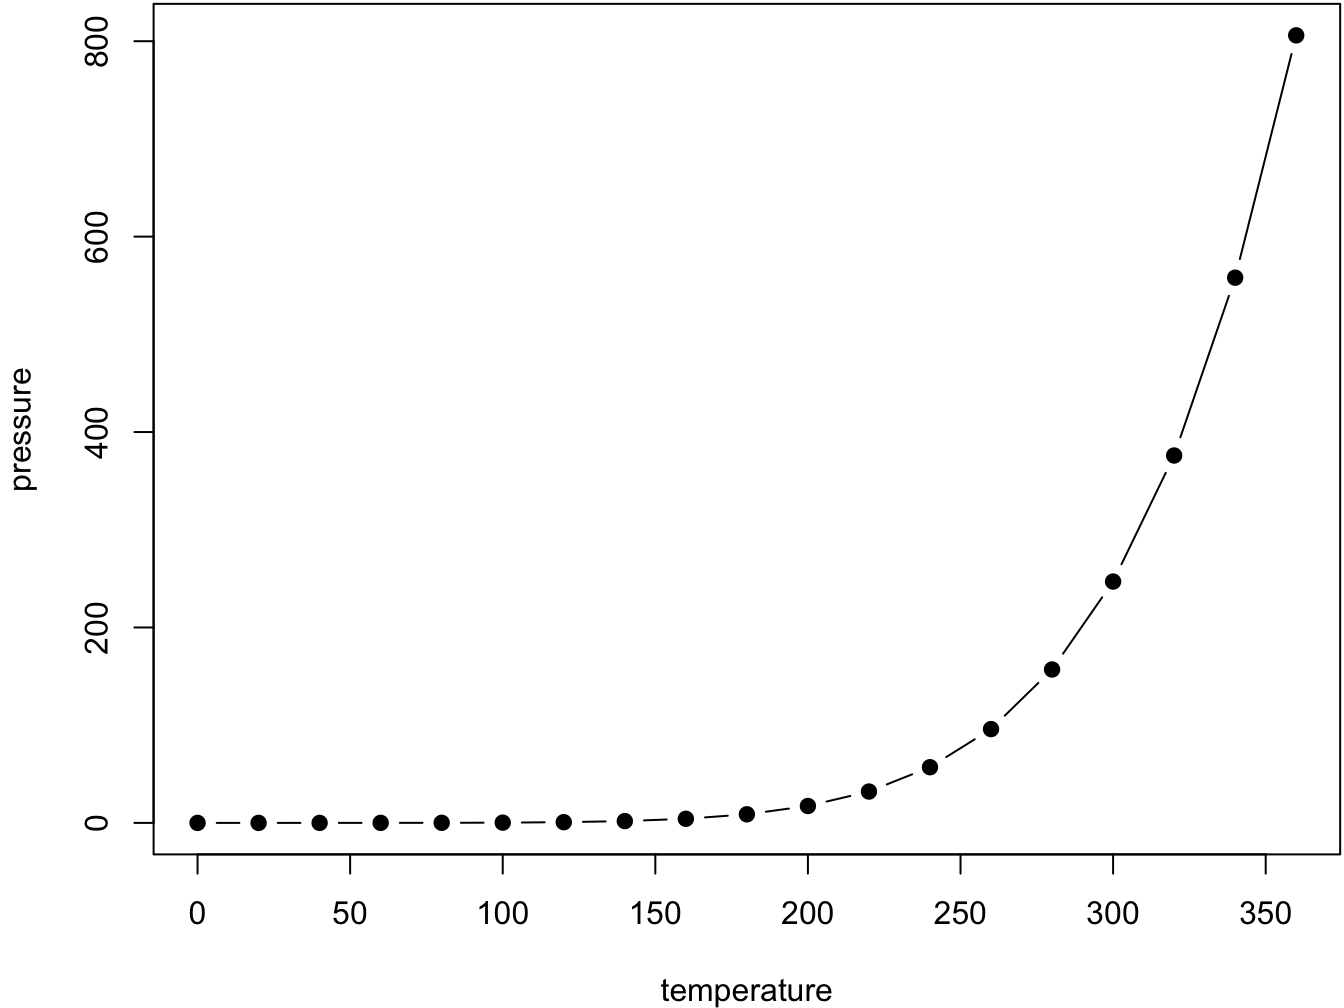
\includegraphics[width=0.8\linewidth]{bst4r_files/figure-latex/nice-fig-1} 

}

\caption{Here is a nice figure!}\label{fig:nice-fig}
\end{figure}

Reference a figure by its code chunk label with the \texttt{fig:}
prefix, e.g., see Figure \ref{fig:nice-fig}. Similarly, you can
reference tables generated from \texttt{knitr::kable()}, e.g., see Table
\ref{tab:nice-tab}.

\begin{Shaded}
\begin{Highlighting}[]
\NormalTok{knitr}\OperatorTok{::}\KeywordTok{kable}\NormalTok{(}
  \KeywordTok{head}\NormalTok{(iris, }\DecValTok{20}\NormalTok{), }\DataTypeTok{caption =} \StringTok{'Here is a nice table!'}\NormalTok{,}
  \DataTypeTok{booktabs =} \OtherTok{TRUE}
\NormalTok{)}
\end{Highlighting}
\end{Shaded}

\begin{table}

\caption{\label{tab:nice-tab}Here is a nice table!}
\centering
\begin{tabular}[t]{rrrrl}
\toprule
Sepal.Length & Sepal.Width & Petal.Length & Petal.Width & Species\\
\midrule
5.1 & 3.5 & 1.4 & 0.2 & setosa\\
4.9 & 3.0 & 1.4 & 0.2 & setosa\\
4.7 & 3.2 & 1.3 & 0.2 & setosa\\
4.6 & 3.1 & 1.5 & 0.2 & setosa\\
5.0 & 3.6 & 1.4 & 0.2 & setosa\\
\addlinespace
5.4 & 3.9 & 1.7 & 0.4 & setosa\\
4.6 & 3.4 & 1.4 & 0.3 & setosa\\
5.0 & 3.4 & 1.5 & 0.2 & setosa\\
4.4 & 2.9 & 1.4 & 0.2 & setosa\\
4.9 & 3.1 & 1.5 & 0.1 & setosa\\
\addlinespace
5.4 & 3.7 & 1.5 & 0.2 & setosa\\
4.8 & 3.4 & 1.6 & 0.2 & setosa\\
4.8 & 3.0 & 1.4 & 0.1 & setosa\\
4.3 & 3.0 & 1.1 & 0.1 & setosa\\
5.8 & 4.0 & 1.2 & 0.2 & setosa\\
\addlinespace
5.7 & 4.4 & 1.5 & 0.4 & setosa\\
5.4 & 3.9 & 1.3 & 0.4 & setosa\\
5.1 & 3.5 & 1.4 & 0.3 & setosa\\
5.7 & 3.8 & 1.7 & 0.3 & setosa\\
5.1 & 3.8 & 1.5 & 0.3 & setosa\\
\bottomrule
\end{tabular}
\end{table}

You can write citations, too. For example, we are using the
\textbf{bookdown} package \citep{R-bookdown} in this sample book, which
was built on top of R Markdown and \textbf{knitr} \citep{xie2015}.

\chapter{Chapter 2: Descriptive
Statistics}\label{chapter-2-descriptive-statistics}

\section{Introduction}\label{introduction}

\section{Measures of Location using Base
R}\label{measures-of-location-using-base-r}

\begin{Shaded}
\begin{Highlighting}[]
\KeywordTok{library}\NormalTok{(xlsx)}

\KeywordTok{head}\NormalTok{(ChickWeight)}
\end{Highlighting}
\end{Shaded}

\begin{verbatim}
  weight Time Chick Diet
1     42    0     1    1
2     51    2     1    1
3     59    4     1    1
4     64    6     1    1
5     76    8     1    1
6     93   10     1    1
\end{verbatim}

\subsection{The Arithmetic Mean}\label{the-arithmetic-mean}

The arithmetic mean is the sum of all the observations divided by the
number of observations. It is written in statistical terms as

\[\overline{x} = \frac{1}{n}\sum^n_{i=1}x_i\]

\begin{Shaded}
\begin{Highlighting}[]
\KeywordTok{mean}\NormalTok{(mtcars}\OperatorTok{$}\NormalTok{mpg)}
\end{Highlighting}
\end{Shaded}

\begin{verbatim}
[1] 20.09062
\end{verbatim}

\subsection{The Median}\label{the-median}

\begin{Shaded}
\begin{Highlighting}[]
\KeywordTok{median}\NormalTok{(mtcars}\OperatorTok{$}\NormalTok{mpg)}
\end{Highlighting}
\end{Shaded}

\begin{verbatim}
[1] 19.2
\end{verbatim}

\chapter{Methods}\label{methods}

We describe our methods in this chapter.

\chapter{Applications}\label{applications}

Some \emph{significant} applications are demonstrated in this chapter.

\section{Example one}\label{example-one}

\section{Example two}\label{example-two}

\chapter{Final Words}\label{final-words}

We have finished a nice book.

\bibliography{book.bib,packages.bib}


\end{document}
